%Packages
\usepackage{graphicx}
\usepackage[dvipsnames]{xcolor}
\usepackage{mathptmx}
\usepackage{titletoc}
\usepackage[top=2cm, left=2cm, right=2cm, bottom=2cm]{geometry}
\usepackage{fancyhdr}
\usepackage{amsmath,amsfonts,amssymb,amsthm}
\usepackage[explicit]{titlesec}
\usepackage{tikz}
\usepackage{mdframed}
\usepackage{wrapfig}
\usepackage[linktoc=all]{hyperref}
\usepackage{makeidx}
\usepackage{eso-pic}
\usepackage{xparse}
\usepackage{pgfplots}
\usepackage{paralist}
\usepackage{bm}

%Setting Images Directory
\graphicspath{{images/}}



%Defining Colors
\definecolor{pinkish}{RGB}{255, 220, 220}
\definecolor{turquoise}{RGB}{0,200,200}
\definecolor{TarletonPurple}{RGB}{79,45,127}
\definecolor{LightBlue}{RGB}{130,240,240}
\definecolor{defnGreen}{RGB}{204,255,229}
\definecolor{ocre}{RGB}{243,102,25}

\definecolor{color1}{RGB}{200, 255, 200}
\definecolor{color2}{RGB}{180, 240, 255}
\definecolor{color3}{RGB}{255, 226, 187}
\definecolor{color4}{RGB}{235, 220, 255}

\definecolor{color11}{RGB}{0, 80, 40}
\definecolor{color22}{RGB}{0, 80, 180}
\definecolor{color33}{RGB}{160, 100, 0}
\definecolor{color44}{RGB}{100, 0, 100}

%Hyper ref stuff
\setcounter{secnumdepth}{0}
\hypersetup{hidelinks,backref=true,pagebackref=true,hyperindex=true,colorlinks=false,breaklinks=true,urlcolor= black,bookmarks=true,bookmarksopen=false,pdftitle={Title},pdfauthor={Author}}


%Index Stuff

\makeindex

%Chapter Heading
\newcommand*\chapterlabel{}
\titleformat{\chapter}
 {\gdef\chapterlabel{}
  \normalfont\sffamily\Huge\bfseries}
 {\gdef\chapterlabel{\thechapter\ }}{0pt}
 {\begin{tikzpicture}[remember picture, overlay]
   \node[yshift=0cm, xshift=10.58cm] at (current page.north west)
     {\begin{tikzpicture}[remember picture, overlay]
       \node{
\includegraphics[width=1.1\paperwidth, height=18cm]{chalk-board-with-math.jpg}} (0,0) rectangle
         (\paperwidth,8cm);
       \draw[anchor=east] node [xshift=8cm,yshift=-7cm, rectangle,
             rounded corners=20pt,inner sep=11pt, draw=black,
             fill=white]
             {\color{black}\chapterlabel#1};
      \end{tikzpicture}
     };
  \end{tikzpicture}
 }
\titlespacing*{\chapter}{0pt}{40pt}{130pt}


%New Commands



%New Theorem Styles

\newtheoremstyle{blacknumbered}% Theorem style name
{5pt}% Space above
{5pt}% Space below
{\large\normalfont}% Body font
{0pt} % Indent amount
{\color{blue}\Large\bf}% Theorem head font
{\\}% Punctuation after theorem head
{6cm}% Space after theorem head
{}

\newtheoremstyle{thedefnone}% Theorem style name
{5pt}% Space above
{5pt}% Space below
{\large\normalfont}% Body font
{0pt} % Indent amount
{\color{color11}\Large\bf}% Theorem head font
{\\}% Punctuation after theorem head
{6cm}% Space after theorem head
{}

\newtheoremstyle{theexmplone}% Theorem style name
{5pt}% Space above
{5pt}% Space below
{\large\normalfont}% Body font
{0pt} % Indent amount
{\color{color44}\Large\bf}% Theorem head font
{\\}% Punctuation after theorem head
{6cm}% Space after theorem head
{}

\newtheoremstyle{thethmone}% Theorem style name
{5pt}% Space above
{5pt}% Space below
{\large\normalfont}% Body font
{0pt} % Indent amount
{\color{color22}\Large\bf}% Theorem head font
{\\}% Punctuation after theorem head
{6cm}% Space after theorem head
{}

\newtheoremstyle{theprblmone}% Theorem style name
{5pt}% Space above
{5pt}% Space below
{\large\normalfont}% Body font
{0pt} % Indent amount
{\color{color33}\Large\bf}% Theorem head font
{\\}% Punctuation after theorem head
{6cm}% Space after theorem head
{}

\newtheoremstyle{exercises}% Theorem style name
{5pt}% Space above
{5pt}% Space below
{\large\normalfont}% Body font
{0pt} % Indent amount
{\Large\bf}% Theorem head font
{ --}% Punctuation after theorem head
{1cm}% Space after theorem head
{}
%Frames for Environments
\newmdenv[skipabove=7pt,
skipbelow=7pt,
rightline=false,
leftline=false,
topline=false,
bottomline=false,
backgroundcolor=color1,
linecolor=red,
innerleftmargin=5pt,
innerrightmargin=5pt,
innertopmargin=5pt,
innerbottommargin=5pt,
leftmargin=0cm,
rightmargin=0cm,
linewidth=8pt]{defnbox}

\newmdenv[skipabove=7pt,
skipbelow=7pt,
rightline=false,
leftline=true,
topline=false,
bottomline=false,
linecolor=red,
innerleftmargin=5pt,
innerrightmargin=5pt,
innertopmargin=5pt,
innerbottommargin=5pt,
leftmargin=0cm,
rightmargin=0cm,
linewidth=8pt]{presentation}

\newmdenv[skipabove=7pt,
skipbelow=7pt,
rightline=false,
leftline=false,
topline=false,
bottomline=false,
backgroundcolor=color3,
linecolor=red,
innerleftmargin=5pt,
innerrightmargin=5pt,
innertopmargin=5pt,
innerbottommargin=5pt,
leftmargin=0cm,
rightmargin=0cm,
linewidth=8pt]{prblmbox}

\newmdenv[skipabove=7pt,
skipbelow=7pt,
rightline=false,
leftline=false,
topline=false,
bottomline=false,
backgroundcolor=color4,
linecolor=red,
innerleftmargin=5pt,
innerrightmargin=5pt,
innertopmargin=5pt,
innerbottommargin=5pt,
leftmargin=0cm,
rightmargin=0cm,
linewidth=8pt]{examplebox}

\newmdenv[skipabove=7pt,
skipbelow=7pt,
rightline=false,
leftline=false,
topline=false,
bottomline=false,
backgroundcolor=color2,
linecolor=red,
innerleftmargin=5pt,
innerrightmargin=5pt,
innertopmargin=5pt,
innerbottommargin=5pt,
leftmargin=0cm,
rightmargin=0cm,
linewidth=8pt]{theorembox}


%New Theorems
\theoremstyle{theprblmone}
\newtheorem{prblmx}[section]{Problem}
\theoremstyle{theexmplone}
\newtheorem{exmpl}[section]{Example}

\theoremstyle{thedefnone}
\newtheorem{defnx}[section]{Definition}
\theoremstyle{thethmone}
\newtheorem{theoremx}[section]{Theorem}
\theoremstyle{plain}
\newtheorem{theoaux}[subsection]{Theorem}
\theoremstyle{exercises}
\newtheorem{exercise}{Ex.}

%New Environments

\newenvironment{defn}
	{\begin{defnbox}
	\begin{defnx}}
	{\end{defnx}
	\end{defnbox}}


\newenvironment{prblm}
	{\begin{prblmbox}
	\begin{prblmx}}
	{\end{prblmx}
	\end{prblmbox}}	

\newenvironment{example}{\begin{examplebox}\begin{exmpl}}{\end{exmpl}\end{examplebox}}

\newenvironment{theorem}{\begin{theorembox}\begin{theoremx}}{\end{theoremx}\end{theorembox}}




	
\newenvironment{WrapBoxR}[1][r]
  {\wrapfigure{#1}{0.5\textwidth}\mdframed[backgroundcolor=LightBlue!30,skipabove=0pt,skipbelow=0pt]}
  {\endmdframed\endwrapfigure}

\newenvironment{WrapBoxL}[1][l]
  {\wrapfigure{#1}{0.5\textwidth}\mdframed[backgroundcolor=LightBlue!30,skipabove=0pt,skipbelow=0pt]}
  {\endmdframed\endwrapfigure}
  

%New Commands

\newcommand{\numline}{\begin{center}
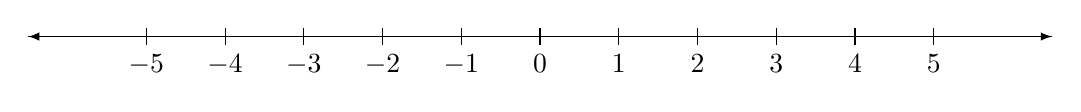
\begin{tikzpicture}
\draw[latex-] (-6.5,0) -- (6.5,0) ;
\draw[-latex] (-6.5,0) -- (6.5,0) ;
\foreach \x in  {-5,-4,-3,-2,-1,0,1,2,3,4,5}
\draw[shift={(\x,0)},color=black] (0pt,3pt) -- (0pt,-3pt);
\foreach \x in {-5,-4,-3,-2,-1,0,1,2,3,4,5 }
\draw[shift={(\x,0)},color=black] (0pt,0pt) -- (0pt,-3pt) node[below] 
{$\x$};
\end{tikzpicture}
\end{center}}

%Pgfplot stuff

\usetikzlibrary{shapes,arrows}
\usetikzlibrary{arrows.meta,positioning,calc}
\pgfplotsset{
    vasymptote/.style={before end axis/.append code={\draw[dashed,<->,-{Latex}] ({rel axis cs:0,0} -| {axis cs:#1,0}) -- ({rel axis cs:0,1} -| {axis cs:#1,0}); }},
    myaxis/.style={axis line style={<->, {Latex}-{Latex}}}
}

